\section{LE6 -- Netzwerk-Kennzahlen}

Netzwerk-Kennzahlen quantifizieren strukturelle Eigenschaften auf Knoten-, Kanten- und Netzwerkebene. Sie ermöglichen systematische Vergleiche zwischen verschiedenen Netzwerken und offenbaren wichtige Muster über Konnektivität, Zentralität, Clustering und die Gesamtarchitektur des Netzwerks. In diesem Kapitel analysieren wir globale und lokale Metriken auf unseren Fussballnetzwerken und interpretieren ihre Bedeutung im taktischen Kontext.

\subsection{Ziel}
\textit{Welche globalen und lokalen Kennzahlen beschreiben das Netzwerk sinnvoll?}

Während LE5 sich auf die Identifikation \textbf{zentraler Aktoren} konzentrierte (wer ist wichtig?), fokussiert sich LE6 auf die \textbf{strukturellen Eigenschaften des Gesamtnetzwerks} (wie ist das Netzwerk aufgebaut?). Die Fragen sind komplementär: Zentralitätsmasse aus LE5 charakterisieren individuelle Knoten, während die hier untersuchten Metriken das kollektive Verhalten und die Netzwerkarchitektur beschreiben.

\textbf{Hinweis:} Mehrere Kennzahlen wurden bereits in vorherigen Kapiteln implementiert:
\begin{itemize}
  \item \textbf{Degree, Strength, Betweenness, Closeness, Eigenvector, PageRank, k-Core} → siehe LE5
  \item \textbf{Dichte, Modularität} → siehe LE4 (Community Detection)
\end{itemize}

Diese Kennzahlen werden hier nicht wiederholt, sondern wir fokussieren uns auf ergänzende Metriken: Diameter, Average Path Length, Clustering Coefficient, Transitivity, Assortativity, Reciprocity und Edge Embeddedness.

\subsection{Datengrundlage}

Wir analysieren zwei Netzwerke:
\begin{itemize}
  \item \textbf{Pass-Netzwerk (Deutschland Bundesliga)}: 473 Knoten (Spieler), 8\,815 gerichtete Kanten (Pässe), gewichtet nach Passanzahl
  \item \textbf{Match-Netzwerk (FIFA World Cup)}: 32 Knoten (Teams), 126 gerichtete Kanten (Spiele), gewichtet nach Toren
\end{itemize}

Für metriken, die Zusammenhang voraussetzen (Diameter, Average Path Length), verwenden wir die \textbf{grösste zusammenhängende Komponente} (Largest Connected Component, LCC):
\begin{itemize}
  \item Pass-Netzwerk LCC: 283 Knoten (59.8\%), 2\,899 Kanten
  \item Match-Netzwerk: vollständig zusammenhängend (1 Komponente)
\end{itemize}

\subsection{Globale Kennzahlen}

\subsubsection{Diameter und Average Path Length}

Der \textbf{Diameter} $D$ ist die maximale kürzeste Pfaddistanz zwischen zwei Knoten:
\begin{equation}
D = \max_{i,j \in V} d(i,j)
\end{equation}

Die \textbf{Average Path Length} $\bar{d}$ ist die durchschnittliche kürzeste Pfaddistanz über alle Knotenpaare:
\begin{equation}
\bar{d} = \frac{1}{n(n-1)} \sum_{i \neq j} d(i,j)
\end{equation}

wobei $d(i,j)$ die kürzeste Pfaddistanz zwischen Knoten $i$ und $j$ ist.

\paragraph{Ergebnisse}

\begin{table}[h]
\centering
\caption{Diameter und Average Path Length}
\label{tab:diameter_path_length}
\begin{tabular}{lcc}
\toprule
\textbf{Netzwerk} & \textbf{Diameter} & \textbf{Avg Path Length} \\
\midrule
Pass-Netzwerk (LCC) & 13 & 5.476 \\
Match-Netzwerk & 6 & 3.163 \\
\bottomrule
\end{tabular}
\end{table}

\textbf{Interpretation:}
\begin{itemize}
  \item \textbf{Pass-Netzwerk}: Spieler sind im Durchschnitt 5.5 Passschritte voneinander entfernt. Der Diameter von 13 zeigt, dass einige periphere Spieler (vermutlich Ersatzspieler oder Spezialisten) weit vom Kern des Passnetzes entfernt sind.
  \item \textbf{Match-Netzwerk}: Teams sind durchschnittlich 3.2 Schritte auseinander. Der Diameter von 6 reflektiert die K.O.-Struktur (Gruppenphase → Finale).
\end{itemize}

\paragraph{Small-World-Eigenschaft}
Netzwerke zeigen die Small-World-Eigenschaft, wenn $\bar{d} \sim \log(n)$ (logarithmische Skalierung mit Netzwerkgrösse). Überprüfung:

\begin{table}[h]
\centering
\caption{Small-World-Check}
\label{tab:small_world_check}
\begin{tabular}{lccc}
\toprule
\textbf{Netzwerk} & \textbf{$\bar{d}$} & \textbf{$\log(n)$} & \textbf{Ratio} \\
\midrule
Pass-Netzwerk & 5.476 & 5.645 & 0.97 \\
Match-Netzwerk & 3.163 & 3.466 & 0.91 \\
\bottomrule
\end{tabular}
\end{table}

Beide Netzwerke erfüllen die Small-World-Eigenschaft (Ratio $\approx 1$): Sie zeigen effiziente Pfadlängen trotz ihrer unterschiedlichen Grössen. Im Pass-Netzwerk bedeutet dies, dass der Ball durch gut organisierte taktische Positionierung schnell über das gesamte Team fliessen kann.

\subsubsection{Clustering Coefficient und Transitivity}

Der \textbf{lokale Clustering-Koeffizient} $C_i$ misst, wie stark die Nachbarn eines Knotens $i$ untereinander vernetzt sind:
\begin{equation}
C_i = \frac{2e_i}{k_i(k_i-1)}
\end{equation}

wobei $e_i$ die Anzahl der Kanten zwischen den Nachbarn von $i$ ist und $k_i$ der Grad von $i$.

Der \textbf{durchschnittliche Clustering-Koeffizient} ist:
\begin{equation}
\bar{C} = \frac{1}{n} \sum_{i=1}^{n} C_i
\end{equation}

Die \textbf{Transitivity} (globaler Clustering-Koeffizient) misst die Gesamtdichte an Dreiecken:
\begin{equation}
C_{global} = \frac{3 \times \text{Anzahl Dreiecke}}{\text{Anzahl verbundener Tripel}}
\end{equation}

\paragraph{Ergebnisse}

\begin{table}[h]
\centering
\caption{Clustering-Metriken}
\label{tab:clustering_metrics}
\begin{tabular}{lccc}
\toprule
\textbf{Netzwerk} & \textbf{$\bar{C}$} & \textbf{Transitivity} & \textbf{Dreiecke} \\
\midrule
Pass-Netzwerk (LCC) & 0.8667 & 0.8183 & 17\,093 \\
Match-Netzwerk & 0.7003 & 0.4904 & 34 \\
\bottomrule
\end{tabular}
\end{table}

\begin{figure}[h]
  \centering
  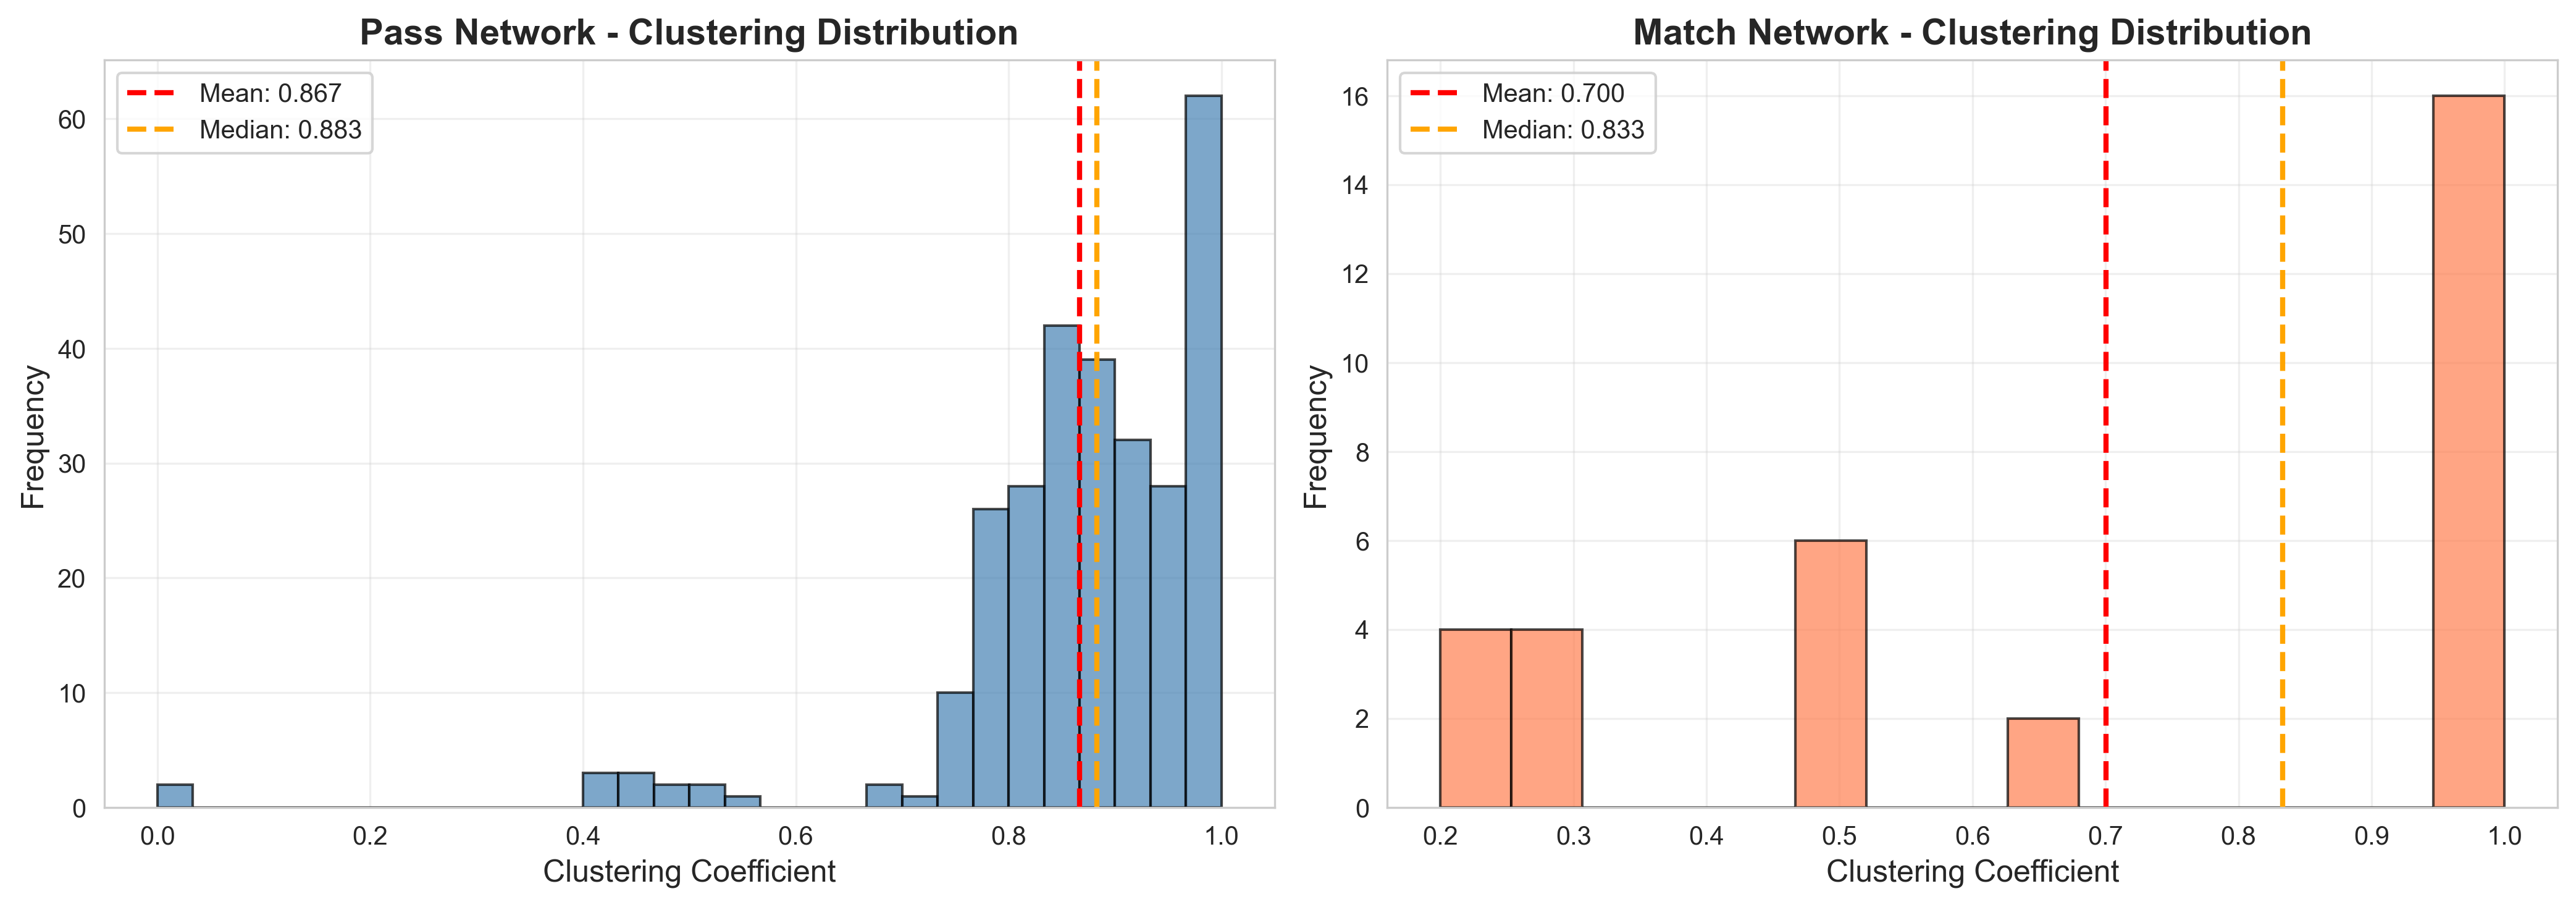
\includegraphics[width=0.95\linewidth]{figures/LE6/clustering_distribution.png}
  \caption{Verteilung des Clustering-Koeffizienten. Links: Pass-Netzwerk (hoch konzentriert um 0.8 - 0.9). Rechts: Match-Netzwerk (variierter).}
  \label{fig:clustering_distribution}
\end{figure}

\textbf{Interpretation:}
\begin{itemize}
  \item \textbf{Pass-Netzwerk}: Aussergewöhnlich hoher durchschnittlicher Clustering-Koeffizient (0.867) zeigt, dass Spieler in \textbf{eng vernetzten taktischen Einheiten} operieren. 81.6\% der Spieler haben $C_i \geq 0.8$, viele erreichen perfektes Clustering ($C_i = 1.0$). Dies reflektiert Positionsgruppen wie Verteidigungslinien oder Mittelfeld-Dreiecke.
  \item \textbf{Match-Netzwerk}: Hoher durchschnittlicher Clustering (0.700) reflektiert die Gruppenphase, in der Teams innerhalb einer Gruppe alle gegeneinander spielen.
\end{itemize}

\paragraph{Vergleich mit Zufallsnetzwerken}
In einem Zufallsnetzwerk mit gleicher Dichte gilt $C_{random} \approx \rho$ (Dichte). Vergleich:

\begin{table}[h]
\centering
\caption{Clustering vs. Zufallsnetzwerk}
\label{tab:clustering_vs_random}
\begin{tabular}{lccc}
\toprule
\textbf{Netzwerk} & \textbf{Clustering} & \textbf{Dichte} & \textbf{Ratio} \\
\midrule
Pass-Netzwerk & 0.8183 & 0.0727 & 11.26$\times$ \\
Match-Netzwerk & 0.4904 & 0.1270 & 3.86$\times$ \\
\bottomrule
\end{tabular}
\end{table}

Beide Netzwerke zeigen deutlich höheres Clustering als erwartet: Das Pass-Netzwerk hat \textbf{11.26-fach} höheres Clustering als ein äquivalentes Zufallsnetzwerk. Dies bestätigt stark strukturierte, nicht-zufällige Verbindungsmuster.

\begin{figure}[h]
  \centering
  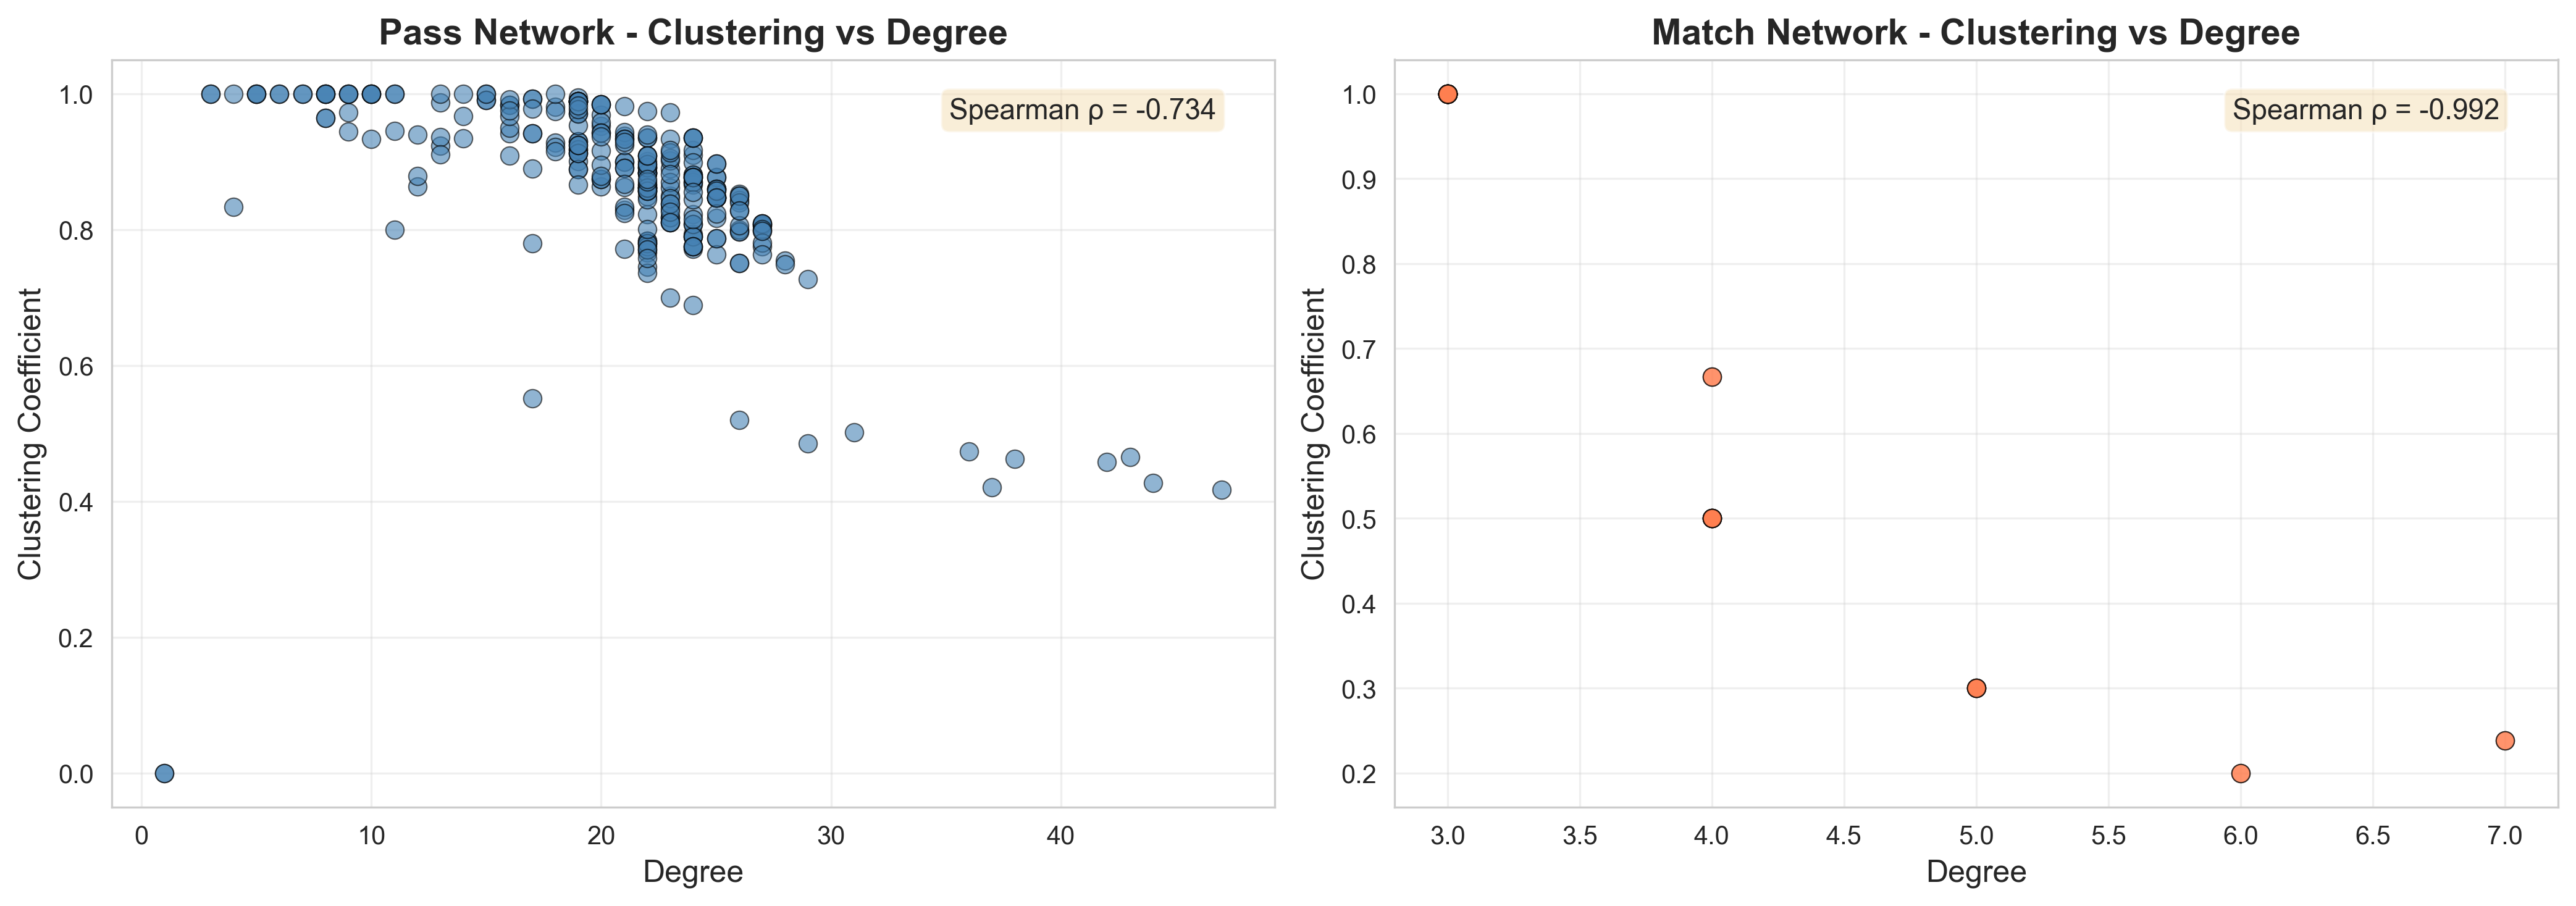
\includegraphics[width=0.95\linewidth]{figures/LE6/clustering_vs_degree.png}
  \caption{Clustering-Koeffizient vs. Degree. Pass-Netzwerk zeigt schwache negative Korrelation (Spearman $\rho = -0.235$), Match-Netzwerk schwache positive Korrelation ($\rho = 0.107$).}
  \label{fig:clustering_vs_degree}
\end{figure}

Die schwache negative Korrelation im Pass-Netzwerk deutet darauf hin, dass Spieler mit vielen Verbindungen (Hubs) tendenziell verschiedene Gruppen überbrücken und daher niedrigeres lokales Clustering aufweisen.

\paragraph{Small-World-Struktur}
Die Kombination von \textbf{niedrige Dichte} (0.073) + \textbf{hoher Clustering} (0.818) + \textbf{kurze Pfadlängen} (5.5) bestätigt die Small-World-Eigenschaft des Pass-Netzwerks: Spieler operieren in eng vernetzten taktischen Einheiten, während der Ball dennoch effizient über das gesamte Team fliessen kann.

\subsubsection{Assortativity}

\textbf{Assortativity} misst die Tendenz ähnlicher Knoten, sich zu verbinden. Die Degree-Assortativity ist die Pearson-Korrelation der Grade an Kantenendpunkten:
\begin{equation}
r = \frac{\text{cov}(k_i, k_j)}{\sigma_{k_i} \sigma_{k_j}}
\end{equation}

Wertebereich: $[-1, 1]$
\begin{itemize}
  \item $r > 0$: \textbf{Assortativ} (Hubs verbinden sich mit Hubs)
  \item $r < 0$: \textbf{Disassortativ} (Hubs verbinden sich mit peripheren Knoten)
  \item $r \approx 0$: Neutrales Mischen
\end{itemize}

\paragraph{Ergebnisse}

\begin{table}[h]
\centering
\caption{Degree-Assortativity}
\label{tab:assortativity}
\begin{tabular}{lc}
\toprule
\textbf{Netzwerk} & \textbf{Assortativity $r$} \\
\midrule
Pass-Netzwerk (ungerichtet) & 0.0062 \\
Pass-Netzwerk (In-Degree) & 0.0007 \\
Pass-Netzwerk (Out-Degree) & -0.0075 \\
Match-Netzwerk & 0.0891 \\
\bottomrule
\end{tabular}
\end{table}

\textbf{Interpretation:}
\begin{itemize}
  \item Beide Netzwerke zeigen \textbf{neutrales Assortativity} ($r \approx 0$), d.h. keine Präferenz für Verbindungen nach Grad-Ähnlichkeit.
  \item \textbf{Pass-Netzwerk}: Anders als in sozialen Netzwerken (oft assortativ, $r > 0.2$) zeigen Fussballteams keine Präferenz für Pässe zwischen Spielern ähnlichen Grades. Schlüsselspieler (Playmaker) passen sowohl zu anderen Kernspielern als auch zu peripheren Angreifern/Verteidigern, funktionale Integration statt Homophilie.
  \item \textbf{Match-Netzwerk}: Leicht positiv (0.089), aber neutral. Reflektiert Balance zwischen Gru\-ppenphase (gemischte Team-Stärken) und K.O.-Runden (ähnliche Performance-Level).
\end{itemize}

Vergleich mit anderen Netzwerktypen:
\begin{itemize}
  \item Soziale Netzwerke: typisch $r > 0.2$ (assortativ)
  \item Technologische Netzwerke: typisch $r < -0.2$ (disassortativ, Hub-and-Spoke)
  \item Fussballnetzwerke: $r \approx 0$ (aufgabenorientiert, keine Grad-Homophilie)
\end{itemize}

\subsubsection{Reciprocity}

\textbf{Reciprocity} $\rho_{recip}$ misst den Anteil bidirektionaler Kanten in gerichteten Netzwerken:
\begin{equation}
\rho_{recip} = \frac{|\{(i,j) : (i,j) \in E \land (j,i) \in E\}|}{|E|}
\end{equation}

Wertebereich: $[0, 1]$

\paragraph{Ergebnisse}

\begin{table}[h]
\centering
\caption{Reciprocity in gerichteten Netzwerken}
\label{tab:reciprocity}
\begin{tabular}{lccc}
\toprule
\textbf{Netzwerk} & \textbf{Reciprocity} & \textbf{Reziproke Kanten} & \textbf{Einseitige Kanten} \\
\midrule
Pass-Netzwerk (LCC) & 0.9269 & 5\,008 (92.7\%) & 395 (7.3\%) \\
Match-Netzwerk & 1.0000 & 126 (100\%) & 0 (0\%) \\
\bottomrule
\end{tabular}
\end{table}

\textbf{Interpretation:}
\begin{itemize}
  \item \textbf{Pass-Netzwerk}: Aussergewöhnlich hohe Reciprocity (92.7\%) zeigt, dass fast alle Passbeziehungen bidirektional sind. Dies reflektiert \textbf{kollaboratives, ballbesitzorientiertes Spiel}, in dem Spieler sich gegenseitig unterstützen. Die wenigen einseitigen Kanten (7.3\%) sind vermutlich spezialisierte Rollen (z.B. Zielspieler empfangen, passen aber selten zurück).
  \item \textbf{Match-Netzwerk}: Perfekte Reciprocity (100\%) ist eine strukturelle Eigenschaft: Jedes Spiel erzeugt eine bidirektionale Beziehung (Team A vs. Team B).
\end{itemize}

Vergleich mit anderen gerichteten Netzwerken:
\begin{itemize}
  \item Soziale Netzwerke (Twitter Follows): 20 - 40\% Reciprocity
  \item Informationsnetzwerke (Web Links): $<10\%$ Reciprocity
  \item Fussball Pass-Netzwerke: 92.7\% Reciprocity: reflektiert kooperative Natur des Teamsports
\end{itemize}

\subsection{Lokale Kennzahlen}

\subsubsection{Edge Embeddedness}

\textbf{Edge Embeddedness} $emb(i,j)$ zählt die gemeinsamen Nachbarn zweier verbundener Knoten:
\begin{equation}
emb(i,j) = |N(i) \cap N(j)|
\end{equation}

wobei $N(i)$ die Nachbarschaft von Knoten $i$ ist.

Kanten mit $emb(i,j) = 0$ werden \textbf{Local Bridges} genannt. Sie verbinden Gruppen ohne gemeinsame Nachbarn.

\paragraph{Ergebnisse}

\begin{table}[h]
\centering
\caption{Edge Embeddedness}
\label{tab:edge_embeddedness}
\begin{tabular}{lcccc}
\toprule
\textbf{Netzwerk} & \textbf{Ø Embeddedness} & \textbf{Median} & \textbf{Max} & \textbf{Local Bridges} \\
\midrule
Pass-Netzwerk (LCC) & 17.69 & 18 & 27 & 2 (0.1\%) \\
Match-Netzwerk & 1.62 & 2 & 3 & 12 (19.0\%) \\
\bottomrule
\end{tabular}
\end{table}

\begin{figure}[h]
  \centering
  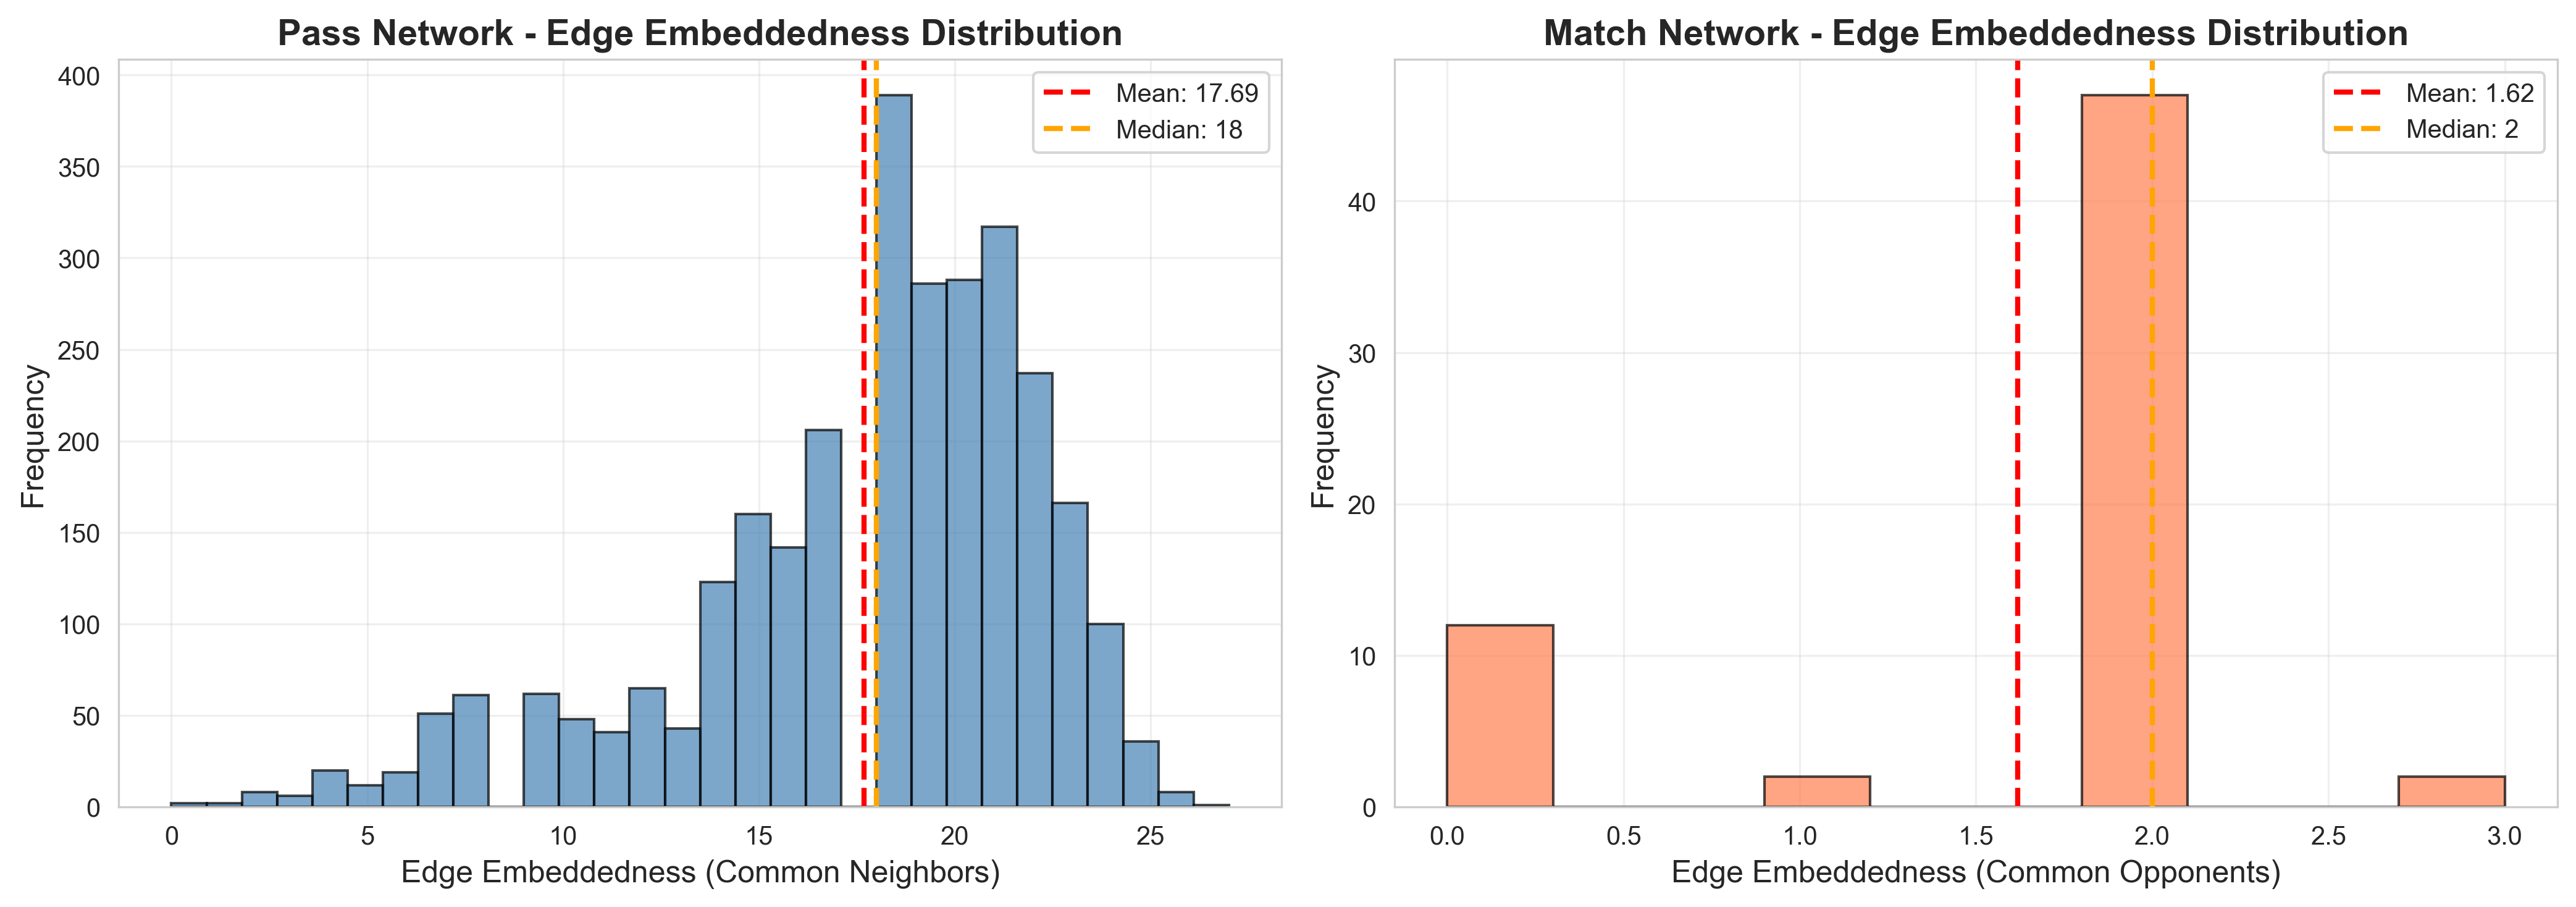
\includegraphics[width=0.95\linewidth]{figures/LE6/edge_embeddedness_distribution.png}
  \caption{Verteilung der Edge Embeddedness. Pass-Netzwerk zeigt hohe Einbettung (Ø 17.7 gemeinsame Nachbarn), Match-Netzwerk niedrige Einbettung (Ø 1.6).}
  \label{fig:edge_embeddedness}
\end{figure}

\textbf{Interpretation:}
\begin{itemize}
  \item \textbf{Pass-Netzwerk}: Aussergewöhnlich hohe Embeddedness (Ø 17.7) zeigt, dass Passbeziehungen \textbf{tief in taktischen Einheiten eingebettet} sind. Verbundene Spieler teilen durchschnittlich 18 gemeinsame Passpartner. Fast keine Local Bridges (nur 2, 0.1\%), praktisch jede Passverbindung hat multiple alternative Routen durch gemeinsame Nachbarn. Dies reflektiert \textbf{redundante taktische Struktur} mit vielfältigen Passoptionen.
  \item \textbf{Match-Netzwerk}: Niedrige Embeddedness (Ø 1.6) reflektiert die begrenzte Verbindung zwischen Turnieren.
  Teams teilen nur 2 gemeinsame Gegner im Durchschnitt. 12 Local Bridges (19\%) repräsentieren Paarungen zwischen Teams aus verschiedenen Gruppen oder Turnierphasen ohne Überlappung.
\end{itemize}

Die Verteilung zeigt (siehe Abb.~\ref{fig:edge_embeddedness}):
\begin{itemize}
  \item Pass-Netzwerk: 91.6\% der Kanten haben $emb \geq 10$, hochredundante Struktur
  \item Match-Netzwerk: Maximum nur 3 gemeinsame Gegner, strukturell begrenzte Überlappung
\end{itemize}

\subsection{Zusammenfassende Analyse}

\begin{table}[h]
\centering
\caption{Umfassende Netzwerk-Metriken (Zusammenfassung)}
\label{tab:comprehensive_metrics}
\resizebox{\textwidth}{!}{%
\begin{tabular}{lcc}
\toprule
\textbf{Metrik} & \textbf{Pass-Netzwerk (LCC)} & \textbf{Match-Netzwerk} \\
\midrule
Knoten & 283 & 32 \\
Kanten & 2\,899 & 63 \\
Dichte & 0.0727 & 0.1270 \\
Diameter & 13 & 6 \\
Avg Path Length & 5.476 & 3.163 \\
Avg Clustering Coef & 0.8667 & 0.7003 \\
Transitivity & 0.8183 & 0.4904 \\
Anzahl Dreiecke & 17\,093 & 34 \\
Avg Edge Embeddedness & 17.69 & 1.62 \\
Assortativity & 0.0062 & 0.0891 \\
Reciprocity & 0.9269 & 1.0000 \\
Small-World Ratio & 0.97 & 0.91 \\
\bottomrule
\end{tabular}%
}
\end{table}

\begin{figure}[h]
  \centering
  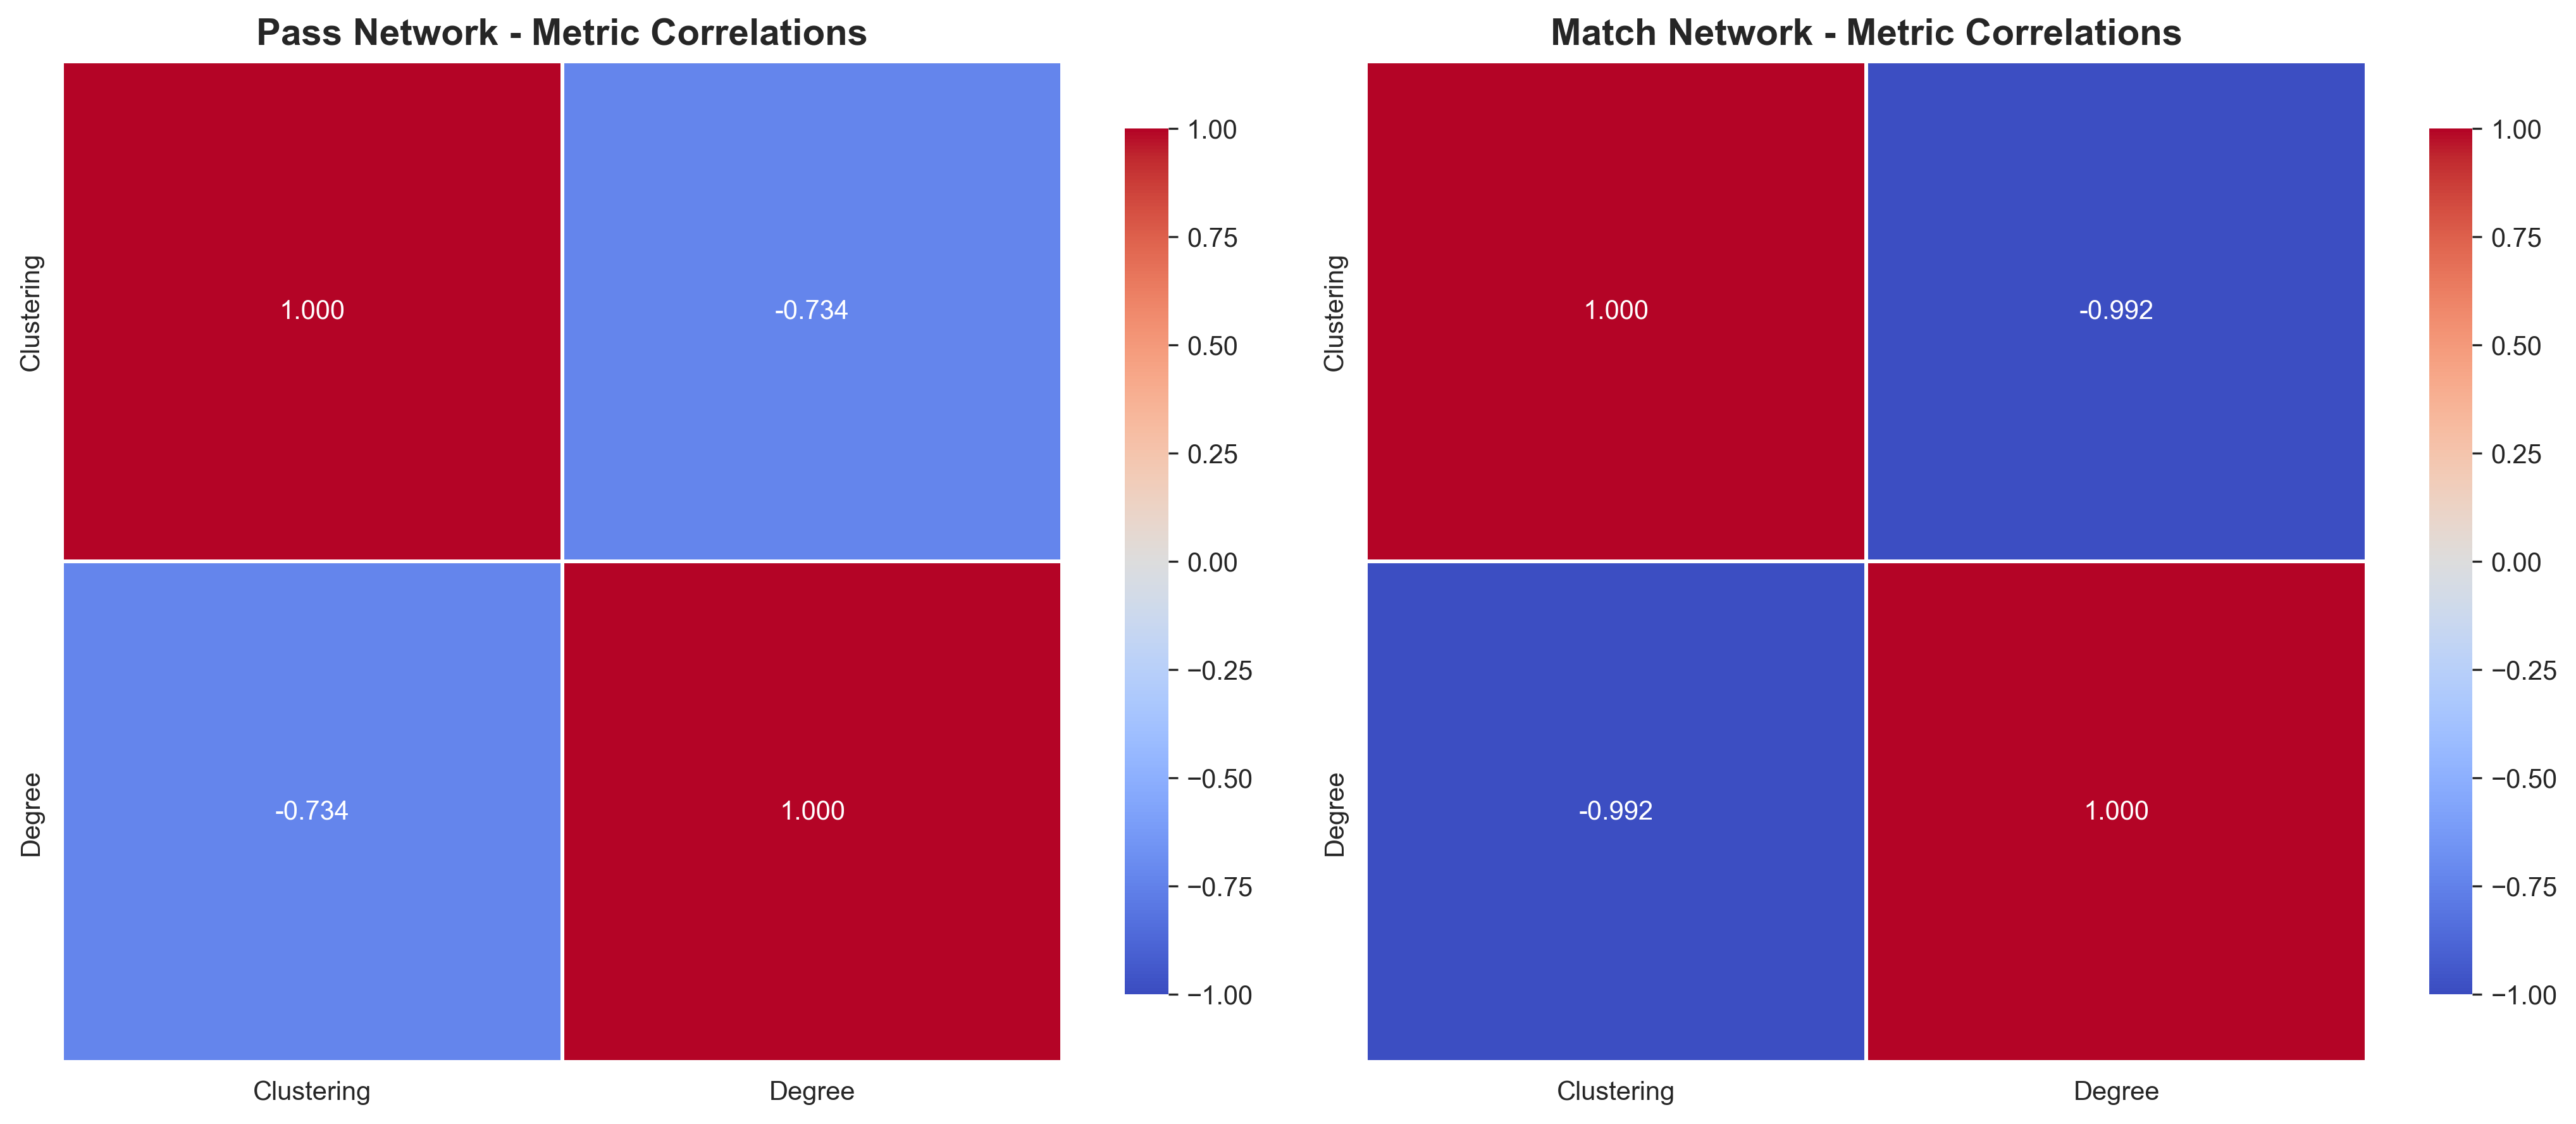
\includegraphics[width=0.8\linewidth]{figures/LE6/metric_correlations.png}
  \caption{Korrelationen zwischen Metriken. Links: Pass-Netzwerk zeigt schwache negative Korrelation zwischen Clustering und Degree ($\rho = -0.235$). Rechts: Match-Netzwerk zeigt schwache positive Korrelation ($\rho = 0.107$).}
  \label{fig:metric_correlations}
\end{figure}

\subsubsection{Strukturelle Unterschiede}

\paragraph{1. Skala \& Konnektivität}
\begin{itemize}
  \item Pass-Netzwerk ist 8.8-fach grösser (283 vs. 32 Knoten)
  \item Aber 1.7-fach weniger dicht (0.073 vs. 0.127)
  \item Grössere Netzwerke können niedrigere Dichte mit hoher Konnektivität kombinieren
\end{itemize}

\paragraph{2. Lokale Struktur (Clustering \& Embeddedness)}
\begin{itemize}
  \item Pass-Netzwerk: 1.7-fach höheres Clustering (0.818 vs. 0.490)
  \item Pass-Kanten 10.9-fach stärker eingebettet (17.7 vs. 1.6 gemeinsame Nachbarn)
  \item \textbf{Pass-Netzwerk}: Eng vernetzte taktische Einheiten mit redundanten Verbindungen
  \item \textbf{Match-Netzwerk}: Spärliche Turnierstruktur mit begrenzter Überlappung
\end{itemize}

\paragraph{3. Globale Struktur (Distanz \& Diameter)}
\begin{itemize}
  \item Pass-Netzwerk hat längere Pfade (Ø 5.5 vs. 3.2)
  \item Beide erfüllen Small-World-Eigenschaft (Ratio $\approx 1$)
  \item Effizient trotz unterschiedlicher Grössen
\end{itemize}

\paragraph{4. Mischungsmuster}
\begin{itemize}
  \item Beide zeigen neutrales Assortativity ($\approx 0$): keine Grad-Homophilie
  \item Beide zeigen hohe Reciprocity (92.7\% Pass, 100\% Match)
  \item \textbf{Pass-Netzwerk}: Kollaboratives ballbesitzorientiertes Spiel
  \item \textbf{Match-Netzwerk}: Round-Robin-Turnierstruktur
\end{itemize}

\paragraph{5. Netzwerktypen}
\begin{itemize}
  \item \textbf{Pass-Netzwerk}: Small-World mit hohem Clustering + niedriger Dichte
  \item \textbf{Match-Netzwerk}: Dichter Turniergraph mit moderatem Clustering
\end{itemize}

\subsection{Diskussion}

\subsubsection{Small-World-Eigenschaften in Fussballnetzwerken}

Die Analyse bestätigt, dass beide Netzwerke \textbf{Small-World-Eigenschaften} aufweisen: kurze Pfadlängen (Effizienz) kombiniert mit hohem Clustering (lokale Struktur). Diese Kombination ist charakteristisch für gut organisierte Systeme.

Im \textbf{Pass-Netzwerk} bedeutet dies:
\begin{itemize}
  \item Spieler operieren in eng vernetzten taktischen Einheiten (Verteidigung, Mittelfeld, Angriff)
  \item Gleichzeitig ermöglicht die Gesamtstruktur schnellen Ballfluss über das gesamte Team
  \item Niedriger Diameter trotz hohem Clustering, optimale Balance zwischen Spezialisierung und Integration
\end{itemize}

\subsubsection{Taktische Implikationen}

Die Metriken offenbaren wichtige taktische Muster:

\paragraph{Redundante Passoptionen}
Hohe Edge Embeddedness (Ø 17.7 gemeinsame Nachbarn) zeigt, dass Teams \textbf{multiple Passoptionen} aufbauen. Wenn ein direkter Pass blockiert ist, existieren viele alternative Routen durch gemeinsame Nachbarn. Dies ist charakteristisch für Ballbesitz-orientierte Taktiken (z.B. Tiki-Taka).

\paragraph{Kollaboratives Spiel}
Sehr hohe Reciprocity (92.7\%) bestätigt, dass erfolgreiches Passspiel auf \textbf{gegenseitiger Unterstützung} basiert. Spieler bieten sich kontinuierlich als Anspielstationen an und schaffen dadurch natürliche bidirektionale Passoptionen.

\paragraph{Funktionale Integration}
Neutrales Assortativity ($r \approx 0$) zeigt, dass Schlüsselspieler (hoher Degree) nicht präferenziell untereinander passen, sondern das gesamte Team integrieren. Dies unterscheidet Fussball von sozialen Netzwerken und reflektiert die \textbf{aufgabenorientierte Natur} des Sports.

\subsubsection{Limitationen}

\paragraph{Statische Perspektive}
Alle Metriken basieren auf statischen, aggregierten Netzwerken. Dynamische Aspekte (wie sich Metriken während eines Spiels ändern) werden nicht erfasst.

\paragraph{Passempfänger-Identifikation}
Unsere Passempfänger-Zuordnung basiert auf raum-zeitlichem Matching (nächster Spieler innerhalb 5 Sekunden, 10 Meter). Fehlzuordnungen können Metriken beeinflussen, insbesondere:
\begin{itemize}
  \item Clustering könnte leicht überschätzt sein (falsche Dreiecke)
  \item Reciprocity robust (aggregierte Muster weniger anfällig)
\end{itemize}

\paragraph{Qualitative Aspekte}
Metriken berücksichtigen nicht die \textbf{Qualität} von Aktionen:
\begin{itemize}
  \item Erfolgreiche vs. erfolglose Pässe
  \item Pässe unter Druck vs. freie Pässe
  \item Rückwärtspässe vs. progressive Pässe
\end{itemize}

\subsection{Fazit}

Die Netzwerk-Kennzahlen offenbaren fundamentale strukturelle Eigenschaften unserer Fussballnetzwerke:

\begin{enumerate}
  \item \textbf{Small-World-Struktur}: Beide Netzwerke kombinieren kurze Pfadlängen (Effizienz) mit hohem Clustering (lokale Struktur)
  \item \textbf{Taktische Organisation}: Aussergewöhnlich hoher Clustering (0.818) und Embeddedness (17.7) zeigen eng vernetzte taktische Einheiten
  \item \textbf{Redundanz}: Multiple Passoptionen durch gemeinsame Nachbarn, charakteristisch für Ballbesitz-Taktiken
  \item \textbf{Kollaboration}: Sehr hohe Reciprocity (92.7\%) reflektiert gegenseitige Unterstützung im Passspiel
  \item \textbf{Funktionale Integration}: Neutrales Assortativity zeigt aufgabenorientierte Vernetzung ohne Grad-Homophilie
\end{enumerate}

Diese Erkenntnisse sind sowohl für deskriptive Netzwerkanalyse als auch für strategische Überlegungen relevant. Die Metriken ermöglichen quantitative Vergleiche zwischen Teams, Ligen oder taktischen Systemen und können als Basis für Performance-Analysen dienen.

\textbf{Ausblick}: Zukünftige Analysen könnten dynamische Metriken (Veränderung während eines Spiels), positions-spezifische Kennzahlen oder den Einfluss von Metriken auf Spielergebnisse untersuchen.
